\documentclass[9pt]{IEEEtran}

% basic
\usepackage[english]{babel}
\usepackage{graphicx,epstopdf,fancyhdr,amsmath,amsthm,amssymb,url,array,textcomp,svg,listings,hyperref,xcolor,colortbl,float,gensymb,longtable,supertabular,multicol,placeins}
\usepackage{hyperref}
 % `sumniki' in names
\usepackage[utf8x]{inputenc}

 % search and copy for `sumniki'
\usepackage[T1]{fontenc}
\usepackage{lmodern}
\input{glyphtounicode}
\pdfgentounicode=1
% \usepackage{subfig}
% tidy figures
\graphicspath{{./figures/}}
\DeclareGraphicsExtensions{.pdf,.png,.jpg,.eps}

% correct bad hyphenation here
\hyphenation{op-tical net-works semi-conduc-tor trig-gs}

% ============================================================================================

\title{\vspace{0ex} %
% TITLE IN HERE:
Navigating the government website network using parallel breadth-first crawler
\\ \normalsize{Web Information Extraction and Retrieval 2018/19, Faculty of Computer and Information Science, University of Ljubljana}}
\author{ %
% AUTHOR IN HERE:
Matej Klemen, Andraž Povše, Jaka Stavanja
\vspace{-4.0ex}
}

% ============================================================================================

\begin{document}

\maketitle

\begin{abstract}
BOII
\begin{lstlisting}
***************************************
***************************************
*************/##***********************
*************%%%%**********************
*//*(*********%&&%%%%%*****************
***(%%%%(*/##%&&%%%%&&%%***************
****#//%%%%&&&&%%&&&&%&&%***********,,,
***************/%%&&&&%%%%***,,,,,,,,,,
**,,,,*,,,,,,,,,#%%&&&&&%%%(,,,,,,,,,,,
******,,,*,,,,,,,/#%&&&&&&&%*,,,,,,,,,,
,,,,,,,,,,,,,,,,,,*(%&&&&&&&***,,,,,,,,
,,,,,,,,,,,,,,,,,,,/,/%&&&&&%(,,,,,,,,,
,,,,,,,,,,,,,,,,,,,,(*,%%&/%&%(**,,,,,,
,,,,,,,,,,,,,,,,,,,,,,**#&%&&%%***,,,,,
,,,,,,,*/,,,,,,,,,,,,,,,(#&%&%%%/*,,,,,
,,,,*///(/(/,,,,,,,,,,,,/#(((((((((((**
***/((/(((((((**,,,,,,,(((((((/(((###**
**(((((/#((#(((********/(#(((((((####/*
*((((##########/********(###(((((####//
//(((((#(#((((#//******/(((#(((((####//
\end{lstlisting}
\end{abstract}

\section{Introduction}

A web crawler is a program that visits web pages and downloads them for some purpose.
It begins with some amount of seed URLs, which are put into a frontier.
The crawler then selects a web page from frontier according to some strategy, visits the web page and extracts the web page's content and outgoing links.
The outgoing links are put into the frontier and the content is used for some purpose or stored.
This process is then repeated until a certain stopping criteria is reached (e.g. the frontier being empty) \cite{Manning2008}.
The crawling can also be a continuous process (``without end''), but we do not study these in this project. 

In this project we implement a web crawler that crawls Slovenian government websites. 
We are given a set of 4 government websites and choose additional 5 of them and proclaim them as seed websites, from which we start the crawling.
While crawling these websites, our crawler only follows links to other Slovenian government websites.
The crawler crawls these websites, downloads images and files from them and stores them into a database. 
The crawler visits new links in a breadth-first fashion.
We also implement a method to detect near-duplicate websites based on their content.
For this, we use a locality-sensitive hashing algorithm based on min-hashing \cite{Gionis1999}.

The rest of the report is structured as follows.
In chapter \textbf{TODO} we present \textbf{TODO}.
In chapter \textbf{TODO} we present \textbf{TODO} \ldots
In chapter ~\ref{section:database} we present how the database is built.

\section{Crawler}
In this section we present the architecture of the crawler. 
The full source code is available online \footnote{\url{https://github.com/matejklemen/govrilovic}}.

The crawler consists of multiple components: link, sitemap and robots parser, database manager (and the database itself), content deduplicator and a core unit which uses the other components and adds on top of them to produce a parallel crawler that uses breadth first search to navigate the websites.

It takes 4 parameters in total. These are seed pages, maximum number of workers, maximum crawling depth and a flag, determining whether to get files. 
The first two parameters are self-explanatory.
The maximum crawling depth is optional and specifies at what depth we want our crawler to stop. 
If this parameter is not provided, the crawler will stop when there are no more links being produced.

[\textbf{TODO: describe each component briefly (mention its role).}]




We used Selenium to make requests, because it also renders the Javascript code on the website. It does, however, not include HTTP status code, which is why we also had to make another request to get that information.


EXPLAIN HOW BREADTH FIRST STRATEGY WORKS
The crawler uses (parallel) breadth-first traversal to crawl the websites. Figure \ref{fig:parallel_bfs} shows an example of how work is divided among workers in our implementation.

The master (the initial process) keeps a structure with visited links and links that still need to be visited (frontier).
On each level, the frontier is emptied and the links are divided among workers as evenly as possible.
Each worker keeps a local copy of its visited websites and a local copy of its newly produced links.
Each worker also checks if a newly visited website is present in the global visited structure, but it does not add new links into it as we want to keep the synchronization between threads to a minimum.
We must wait for all the workers to finish so that breadth-first strategy is ensured.
After they are all done, the master collects newly collected links from workers and checks for duplicate links.
It also marks the links from current level as visited.
This process is repeated with the newly collected links, which represent the next level of search process.

\begin{figure}[h] \centering
    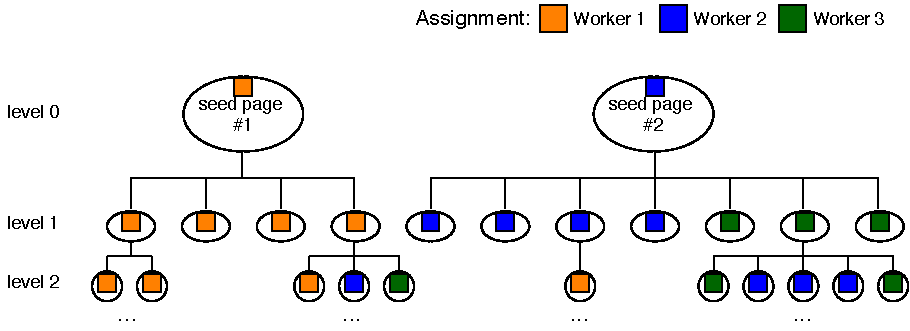
\includegraphics[width=0.45\textwidth]{parallel_bfs.pdf}
    \caption{{How the work is divided among workers in our implementation of parallel breadth-first traversal. The process starts with a set of seed pages, in this case 2. Note that even though we have 3 workers available, we only actually create 2 workers for level 0 as the 3rd one would not receive any work. Workers then gather new outgoing links, which get collected by the master. The work is divided among workers again every time a new level is started.}}
    \label{fig:parallel_bfs}
\end{figure}

We did not use the database as a frontier storage ----- We stored our frontier in the program itself.

\section{Robots and Sitemaps}
Key element of the crawler is also reading the 'robots.txt' file and sitemap. Based on the robots file, we know whether we can visit a certain link or whether it is not allowed for a crawler to visit that link.
We identify our agent as '*' as it is not well known.
What the possibly existent robots file tells us is also the request delay which specifies how much time we have to wait between crawling a page from the same url.
For that reason, we check if either the request delay specified in the 'robots.txt' file or the default delay of 3 seconds has passed to not overload the website we are crawling.
Another thing we can read from the same file is the location of the sitemap.
What we do is we check if there is a sitemap property in the 'robots.txt' file and if there is one, we save its contents to our sitemaps dictionary and the database, else we try and do the same by going to the sites URL and appending it the default sitemap location ('/sitemap.xml').
When we read a sitemap, we add all the URLs mentioned in it, into the frontier. 


\section{Database}\label{section:database}
The database was build inside a Docker container. We used the same schema, with one minor change, which is adding a column 'lsh\_hash' into the page table. The column stores the value that LSH hash produced for the content of that website. Access to database is made by each worker when he visits a new page. The database can handle multiple workers making read and write operations by proper locking of the operations.

For viewing the results and current status in the database, we also used Adminer application, which also runs as a docker container and is then accessable on localhost.


\section{Link}


\section{Image and files extracting}
To work with links correctly, we needed to somehow normalize them.
The first thing we do is we contruct an absolute path for each link, so that we get rid of issues with relative paths.
To do that correctly, we take into consideration the '<base href="somelink">' tags in the webpages, which set the base URL for all the relative paths used in the HTML on the currently crawled webpage.
If there is no base URL on a website, we can treat the URL we are currently crawling as the base one.
What is left is only to append the relative path to the base URL.
The next thing we have to take care of is to get rid of deeply nested URLs to avoid spider traps.
We pass every link through a sanitizer which removes anything after the tenth slash in the URL to avoid looping of URLs.
Then, we sanitize the links further to get rid of any positional arguments after the hash symbol in the url.
We also URL encode the query parameters to prevent different issues which can arise by maybe injecting some malicious code or SQL queries in the URLs.
This encoding also normalizes the capitalization for each URL (the part that is not case sensitive).
We stored images and files into the file system, since it gives a nicer overview of the gathered information. This was made possible by creating a folder for each new site in which we stored the information. We then stored the location of the file/image into the provided data field in the database.




\section{LSH deduplication}
We implemented LSH algorithm, which is being used to compare hashed content of different websites. 

\textbf{How it works}

For the set of words, we hash it on, we used top 1000 Slovenian words. Or maybe triples of characters?


\section{Results - 2 seed URLs}
For the first run of the crawler, we used 2 seed URLs, which were "http://evem.gov.si"and "http://e-prostor.gov.si". We set the maximum crawl depth to None, which means it will run untill there are no more links produced. The maximum number of workers was \textbf{NUM OF WORKERS WE USED}.

The crawling process took XXXX minutes in total and retrieved XXX pages,links, images...

For the sites that are given in the instructions’ seed list and also for the whole crawldb together (for both separately) report general statistics of crawldb (number of sites, number of web pages, number of duplicates, number of binary documents by type, number of images, average number of images per web page, …). Visualize links and include images into the report. If the network is too big, take only a portion of it. Use visualization libraries such as D3js, visjs, sigmajs or gephi.

\section{Results - 9 seed URLs}
The second run consisted of 9 seed urls. For the extra 5 urls of our choice, we have choosen "http://www.mz.gov.si/", "http://www.mnz.gov.si/","http://www.up.gov.si/", "http://www.ti.gov.si/" and "http://www.mf.gov.si/". 




\begin{figure}[h] \centering
    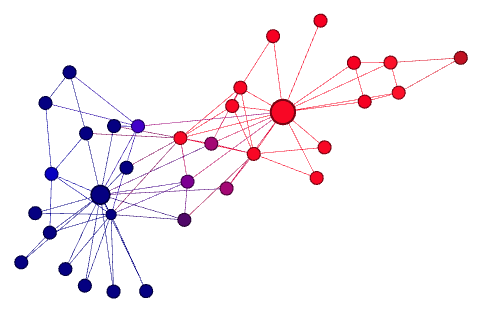
\includegraphics[width=0.4\textwidth]{karate.png}
    \caption{{Example of an image.}}
    \label{fig:karate}
\end{figure}


 
\begin{table}
    \begin{center}
    \caption{Example of a table.}
        \begin{tabular}{ l | r }
        
        Richard Karstark & 0.013661 \\
        Jon Arryn & 0.012869 \\
        Joyeuse Erenford & 0.012869 \\
        Trystane Martell & 0.010761 \\
        Willen Lannister & 0.010684 \\
        Martyn Lannister & 0.010684 \\
        Robb Stark & 0.010304 \\
        Joffrey Baratheon & 0.009875 \\
        Master Caleotte & 0.009495 \\
        Lysa Arryn & 0.009383 \\
        \end{tabular}
    \label{tab:pagerankGOT}
    \end{center}
\end{table}



\bibliographystyle{IEEEtran}
\bibliography{bibliography}


\end{document}
